\documentclass[./../../paper.tex]{subfiles}
\graphicspath{{\subfix{./../../figures/}}}

\begin{document}
\citeauthor{hsieh_DiCE4ELInterpretingProcess_2021} has recently published a paper on the counterfactual generation of process data. They call their framework DiCE4EL and shares many ideas with our framework. Therefore, we want to highlight the key differences and similarities. 

In their approach they attempt to solve various issues that we have also highlighted in \autoref{sec:challenges}. Furthermore, they do so by incrementally generating the model in a sequential order. However, unlike \citeauthor{oberst_CounterfactualOffPolicyEvaluation_2019}, whose solution creates counterfactuals for every step in the sequence, \citeauthor{hsieh_DiCE4ELInterpretingProcess_2021} focus on critical decision points they call milestones. 

To gain a better understanding, it is important to briefly outline the event log the authors use. It was taken from a Dutch bank which processes loan applications in which customers request a certain amount of money. The activities relate to either application states or manual work activities. The application states are basically super tasks generated by a machine and manual work activities produced by humans their substates. Now, to understand why the milestone approach works, requires to know that an application loan process will only be rejected after a manual work item occured. Not, if a the application reaches an application state successfully. Thus, one can split the entire sequence into subsequences, which reducces the search space significantly. 

A crucial distinction to our proposed framework, is their crucial dependence on knowledge about the true process model as displayed in this section. Our framework does not leverage structural information about the true process model in question. We believe this is the core contribution in comparison to their approach.

\begin{figure}[htbp]
    \centering
    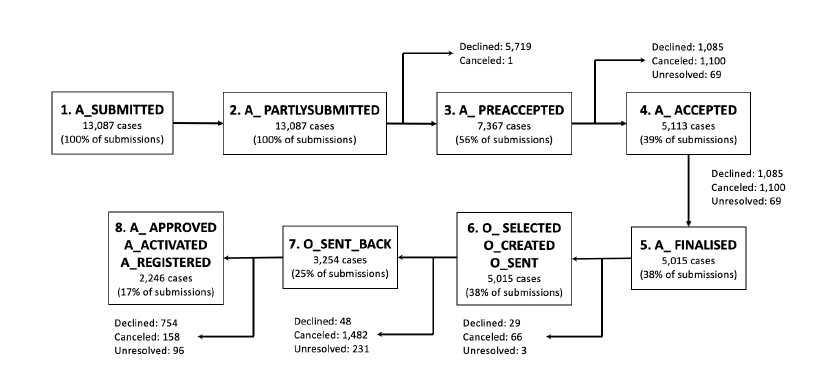
\includegraphics[width=\textwidth]{figures/milestones.png}
    \caption{Milestones of loan application process captured in BPIC2012 as
    identified in \autocite{bautista_ProcessMiningDrivenOptimization_2012}}
    \label{fig:milestones}
\end{figure}

However, similarities between both frameworks do exist. Mainly, our approach also relies on prediction scores of the model we attempt to explain. Similar to \citeauthor{hsieh_DiCE4ELInterpretingProcess_2021}, we incorporate these scores into our quality measure. 

The next difference stems from how DiCE4EL operationalises the quality criteria of their counterfactuals and on what bases they optimize their algorithm. \optional{we will discuss those after discussing our operationalisation in \autoref{sec:viability}}




\end{document}